\def\pgfsysdriver{pgfsys-dvisvgm.def}
\documentclass[tikz,border=8pt]{standalone}
\usepackage{amsmath}
% Semantic palette shared by the light and dark exports; geometry and TeX glyphs stay identical.
\ifdefined\FigureDark
  \definecolor{FigureForeground}{HTML}{E1E8DF}
  \definecolor{FigureMuted}{HTML}{94A69B}
  \definecolor{FigureBlue}{HTML}{8CC5F2}
  \definecolor{FigureOrange}{HTML}{F4B76B}
  \definecolor{FigureRed}{HTML}{F28E86}
  \definecolor{FigureBlueFill}{HTML}{273F4F}
  \definecolor{FigureOrangeFill}{HTML}{4A3726}
  \definecolor{FigurePaper}{HTML}{1B2420}
\else
  \definecolor{FigureForeground}{HTML}{202C29}
  \definecolor{FigureMuted}{HTML}{68766E}
  \definecolor{FigureBlue}{HTML}{245A88}
  \definecolor{FigureOrange}{HTML}{986000}
  \definecolor{FigureRed}{HTML}{A44030}
  \definecolor{FigureBlueFill}{HTML}{E5EDF8}
  \definecolor{FigureOrangeFill}{HTML}{FFF0D8}
  \definecolor{FigurePaper}{HTML}{FBFAF7}
\fi

\begin{document}
% Deficit delta=24 degrees.  The retained sector has angle 336 degrees.
% Isometric development: s=sin(alpha)=336/360; c=cos(alpha).
% F(r,theta)=(s*r*cos(phi),s*r*sin(phi),c*(2-r)),
% phi=(theta-15)/s-70 degrees. Orthographic view: (X,Y,Z)->(X,sin(12)Y+cos(12)Z).
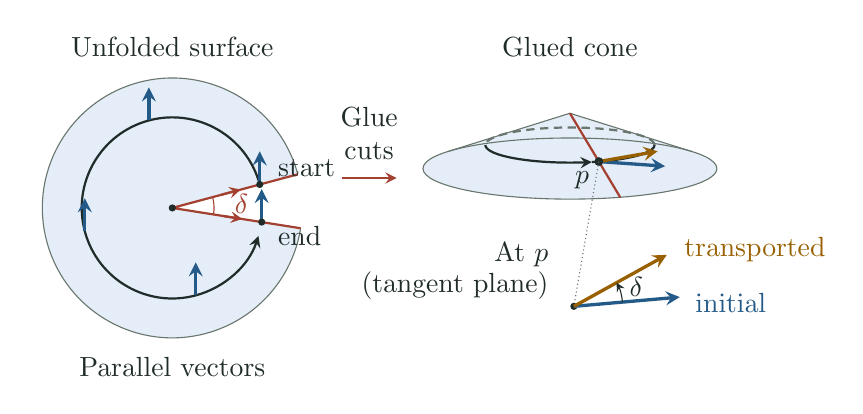
\begin{tikzpicture}[>=stealth,color=FigureForeground,font=\normalsize]
\def\s{0.9333333333}\def\c{0.3590109871}
\def\sy{0.2079116908}\def\sz{0.9781476007}
\node at (0,2.05) {\textnormal{Unfolded surface}};
\fill[FigureBlueFill] (0,0)--(15:1.65) arc(15:351:1.65)--cycle;
\draw[FigureMuted] (15:1.65) arc(15:351:1.65);
\draw[FigureRed,thick] (0,0)--(15:1.65) (0,0)--(351:1.65);
% Matching outward chevrons identify the full radial cuts.
\foreach \a in {15,351}{\draw[FigureRed,thick,->] (\a:.65)--(\a:.9);}
\draw[FigureRed] (351:.53) arc(351:375:.53);
\node[FigureRed] at (.88,.045) {$\delta$};
\draw[->,thick] (15:1.15) arc(15:342:1.15);
\foreach \a in {15,105,195,285,351}{
  \draw[->,FigureBlue,very thick] (\a:1.15)--++(0,.42);
}
\fill (15:1.15) circle(1.3pt);
\fill (351:1.15) circle(1.3pt);
\node[anchor=west] at (1.22,.51) {\textnormal{start}};
\node[anchor=west] at (1.22,-.35) {\textnormal{end}};
\fill (0,0) circle(1.3pt);
\node at (0,-2.02) {\textnormal{Parallel vectors}};
\ifdefined\FigureStacked
\draw[->,FigureRed,thick] (0,-2.38)--(0,-2.92);
\node[anchor=west] at (.18,-2.65) {\textnormal{Glue cuts}};
\begin{scope}[yshift=-4.65cm]
\else
\draw[->,FigureRed,thick] (2.15,.38)--(2.85,.38);
\node[align=center] at (2.5,.95) {\textnormal{Glue}\\\textnormal{cuts}};
\begin{scope}[xshift=5.05cm,yshift=.50cm]
\fi
\node at (0,1.55) {\textnormal{Glued cone}};
% A projected cone with the same slant radius and deficit as the development.
% Apparent generators are tangent to the projected rim: sin(phi)=s*tan(12)/c.
\pgfmathsetmacro{\sil}{asin(\s*\sy/(\c*\sz))}
\fill[FigureBlueFill] (0,{2*\c*\sz})
 --({2*\s*cos(\sil)},{2*\s*\sy*sin(\sil)})
 arc[start angle=\sil,end angle={-180-\sil},x radius={2*\s},y radius={2*\s*\sy}]
 --cycle;
\draw[FigureMuted] (0,{2*\c*\sz})--({2*\s*cos(\sil)},{2*\s*\sy*sin(\sil)})
 (0,{2*\c*\sz})--({-2*\s*cos(\sil)},{2*\s*\sy*sin(\sil)});
\draw[FigureMuted] (0,0) ellipse[x radius={2*\s},y radius={2*\s*\sy}];
% The identified radial cut becomes one seam on the cone.
\draw[FigureRed,thick] (0,{2*\c*\sz})--({2*\s*cos(-70)},{2*\s*\sy*sin(-70)});
% r=1.15 is a closed curve. Rear and front parts have distinct depth treatment.
\draw[densely dashed,FigureMuted,thick,domain=0:180,samples=65]
 plot ({1.15*\s*cos(\x)},{1.15*\s*\sy*sin(\x)+.85*\c*\sz});
\draw[->,thick,domain=180:285,samples=45]
 plot ({1.15*\s*cos(\x)},{1.15*\s*\sy*sin(\x)+.85*\c*\sz});
\draw[thick,domain=285:360,samples=35]
 plot ({1.15*\s*cos(\x)},{1.15*\s*\sy*sin(\x)+.85*\c*\sz});
\coordinate (p) at ({1.15*\s*cos(-70)},{1.15*\s*\sy*sin(-70)+.85*\c*\sz});
% Tangent vectors are pushforwards of their planar counterparts, not overlay arrows.
\foreach \a/\col in {75/FigureBlue,99/FigureOrange}{
 \draw[->,very thick,\col] (p)--++
 ({.85*(cos(\a)*\s*cos(-70)-sin(\a)*sin(-70))},
 {.85*(cos(\a)*(\sy*\s*sin(-70)-\sz*\c)+sin(\a)*\sy*cos(-70))});
}
\fill (p) circle(1.6pt);
\node[anchor=north east] at (p) {$p$};
% An intrinsic tangent-plane enlargement supplies the actual angle comparison.
\draw[FigureMuted,densely dotted] (p)--(.05,-1.75);
\node[anchor=east] at (-.15,-1.10) {\textnormal{At }$p$};
\node[anchor=east] at (-.15,-1.48) {\textnormal{(tangent plane)}};
\begin{scope}[xshift=.05cm,yshift=-1.75cm]
\fill (0,0) circle(1.3pt);
\draw[->,very thick,FigureBlue] (0,0)--(5:1.35);
\draw[->,very thick,FigureOrange] (0,0)--(29:1.35);
\draw[->] (5:.62) arc(5:29:.62);
\node at (17:.83) {$\delta$};
\node[anchor=west,FigureBlue] at (1.42,.05) {\textnormal{initial}};
\node[anchor=west,FigureOrange] at (1.28,.72) {\textnormal{transported}};
\end{scope}
\end{scope}
\end{tikzpicture}
\end{document}
